\subsection{Cleaned}

The platforms provide a huge volume of data, since, as mentioned earlier, they collect as much data as possible.
There will be multiple samples containing the specified set of fields. These field sets may be similar to each other but don't need to be identical.
From this data, we need to select the relevant samples, and from these, the fields necessary to represent specific information.

Below we can see examples. The first one is taken from the European open data portal
(https://www.eea.europa.eu/data-and-maps/data/air-pollutant-concentrations-at-station/air-pollutant-concentrations-201) and the second from the North American open data portal
(https://data.cityofnewyork.us/api/views/kku6-nxdu/rows.json?accessType=DOWNLOAD).

\begin{figure}[ht]
    \centering
    \subfigure[EEUU Open Portal. Demographic Statistics By Zip Code]
     {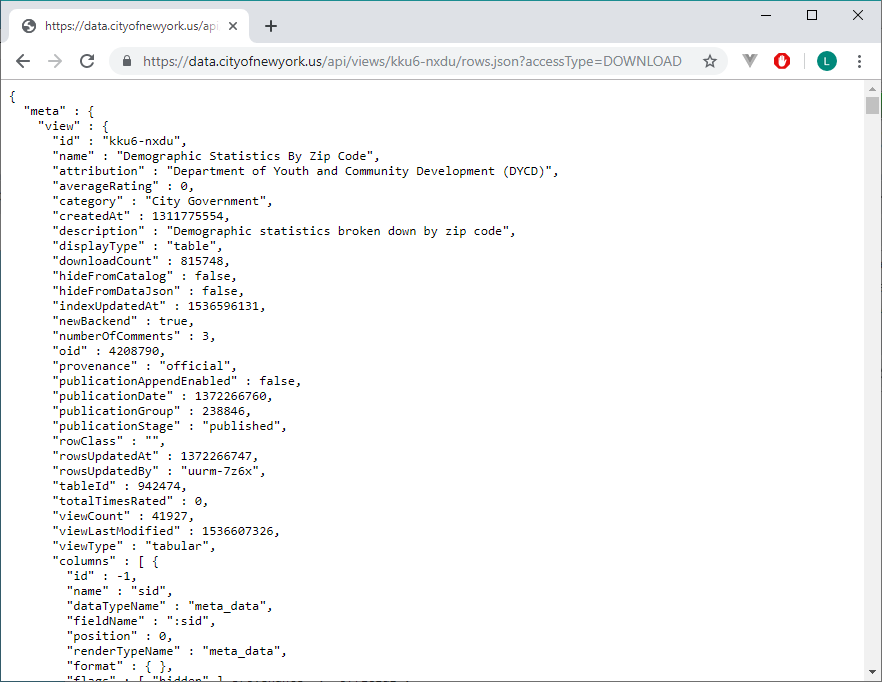
\includegraphics[width=5cm]{ExampleOpenDataEEUU}}
    \hfill
     \subfigure[European Open Data Portal. Air pollutant concentrations 2015]
    {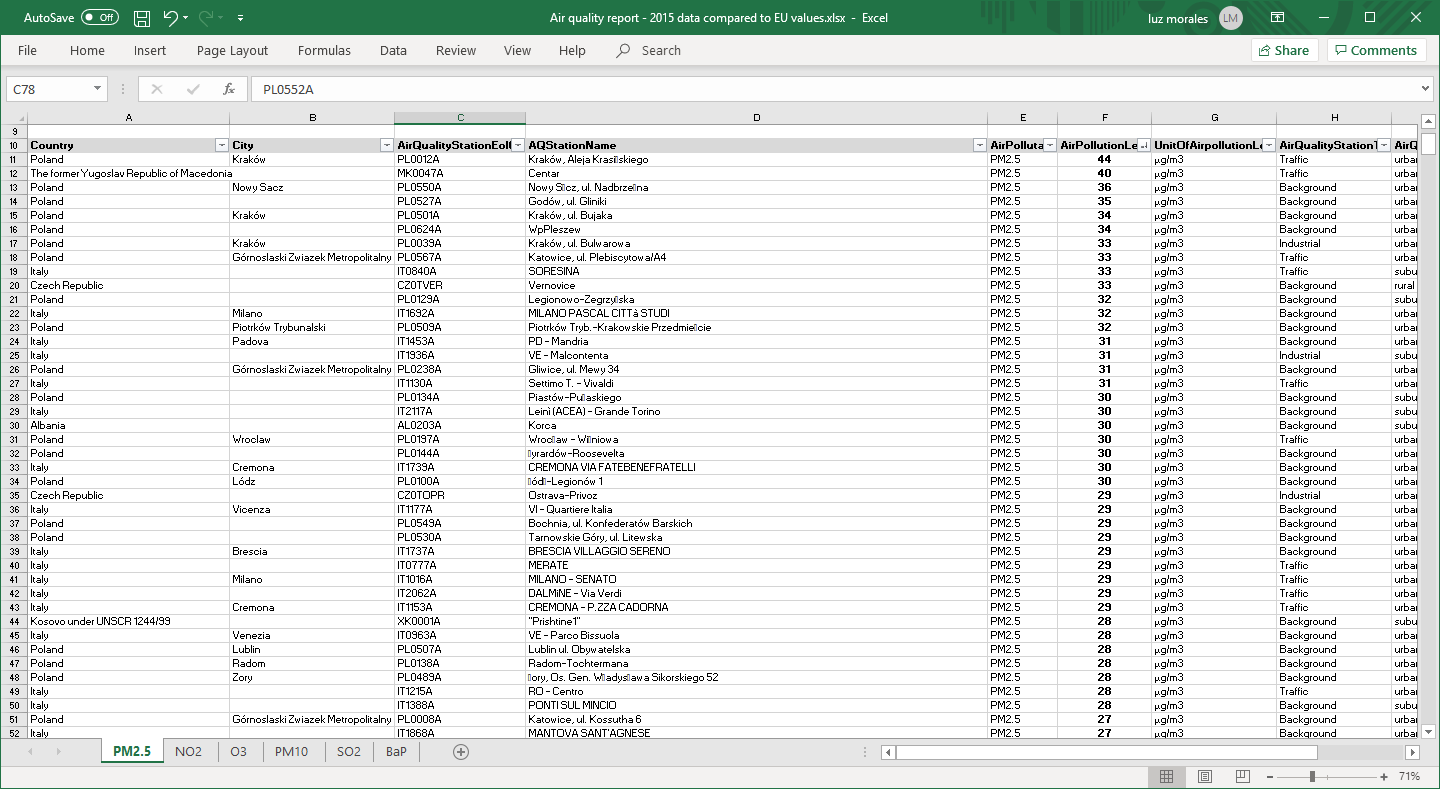
\includegraphics[width=7cm]{ExampleOpenDataEuropean}}
    \caption{Open Data Examples}
\end{figure}
    
\subsubsection*{How to solve it}

We obtain our required data through a series of processes such as extraction, transformation and
cleaning of the data. Without automation, these processes are tedious and time consuming. 

\subsubsection*{How we solve it. Aire Guru} 

The extracted data is in GeoJSON format, a format which provides a JSON object with nested subdocuments. Each of these
subdocuments contains a set of data in key-value form.
In the following figure we can see the beginning of the document downloaded on June 9, 2019
(https://datosabiertos.malaga.eu/recursos/ambiente/calidadaire/calidadaire.json) \\

\begin{figure}[ht]
    \centering
   \subfigure[First subdocument]{ \centering 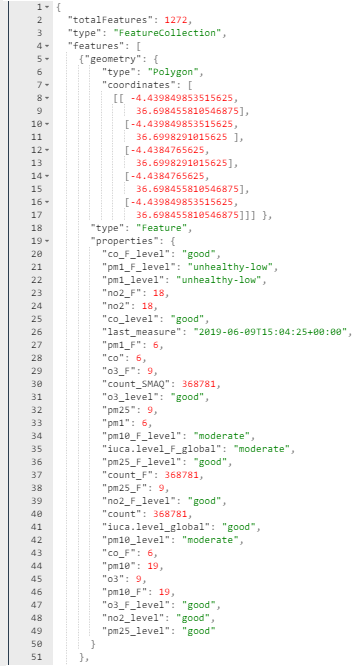
\includegraphics[width=4.75cm]{geoJsonAirQualityData1}}
   \hfill
   \subfigure[Second subdocument]{ \centering 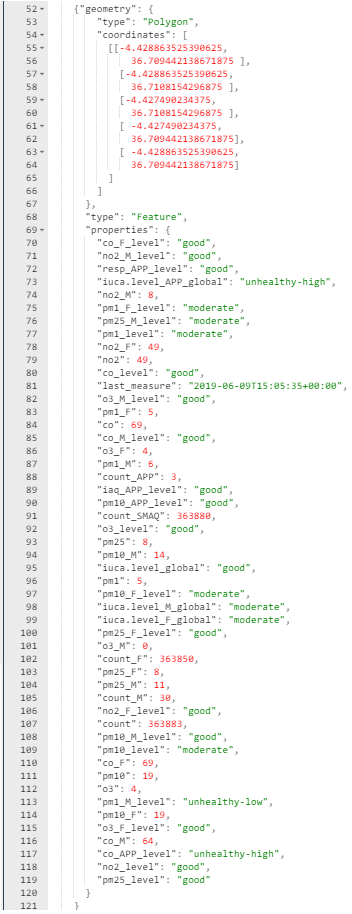
\includegraphics[width=4.75cm]{geoJsonAirQualityData2}}
 
    \caption{Air quality Document [09/06/2019]. Open Data Portal Málaga}
    \end{figure}
    
    In this excerpt we can see the first two subdocuments. Each subdocument contains the coordinates of the air quality 
    measuring station, the date and time when the measurement was recorded, and the values of the measurements.
    In the following figure we can find the description provided by the open data portal.
    
\begin{figure}[ht]
    \centering
    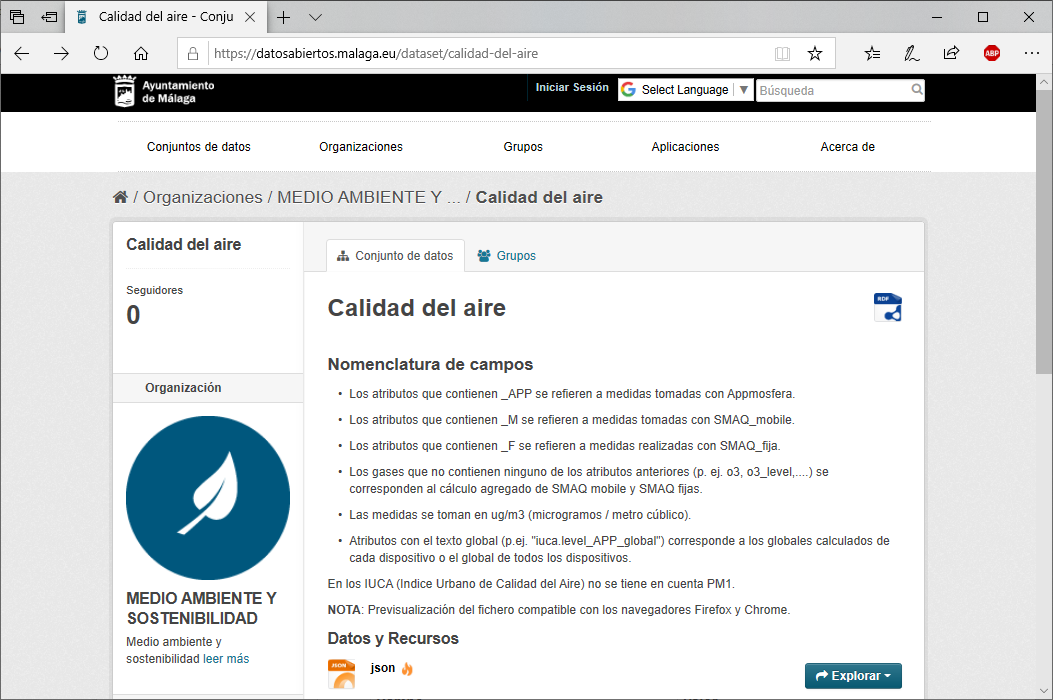
\includegraphics[width=8cm]{geoJsonAirQualityDataDescription}
    \caption{Air quality data description [09/06/2019]. Open Data Portal Málaga}
\end{figure}

For a more detailed description of the measures, we have to resort to an external resource. In this case we directly contacted 
the company that installs the UrbanClouds (https://urbanclouds.city/es/) measuring stations and provides the data 
to the Málaga city council.

After selecting the necessary fields according to our design plan, we carried out different cleaning, transformation and extraction tasks. \\

\textbf{Cleaning}. We need to eliminate the repeated or non-relevant fields. For example, the identifier of the measuring station is 
unneccessary as the  already contains the coordinates of the station, and coordinate representation is more interesting for our purposes. \\

\textbf{Transformation}. We need the values to have a format appropriate to the fields that they represent. For example, the date and time 
of the measurement is stored in date format
instead of the string provided in the raw dataset. \\

\textbf{Extraction}. We need to select the relevant fields. This dataset offers one or more measurements for each pollutant, which can be 
represented by three different fields, a
quantitative measurement, a qualitative of the fixed station of measurement and a qualitative station of a mobile station. We will add a 
field containing the measurement which is most relevant for our purposes, and eliminate the non-relevant measurerments to minimize processing time. \\

For security, a second totally independent architecture has been implemented that collects and stores the raw data.

\paragraph{Evaluation} \mbox{} 

\begin{itemize}
    \done We can understand exactly what each one of the fields represented in the dataset means thanks to the 
         complementary information presented in the open data portal and by the complementary information provided by the company in charge of
         collect the data.
    \done The data needed for our model has been extracted from the raw data.
\end{itemize}